\documentclass[11pt,a4paper]{article}

% ---------- Encodage, langue, police ----------
\usepackage[utf8]{inputenc}
\usepackage[T1]{fontenc}
\usepackage[french]{babel}
\usepackage{lmodern}
\usepackage{microtype}

% ---------- Mise en page ----------
\usepackage[a4paper,margin=2.3cm]{geometry}
\usepackage{parskip}
\usepackage{enumitem}
\setlist{itemsep=2pt,topsep=4pt}

% ---------- Maths, tableaux, figures ----------
\usepackage{amsmath,amssymb}
\usepackage{booktabs}
\usepackage{tabularx}
\usepackage{array}
\usepackage{graphicx}
\usepackage{float}
\usepackage[font=small,labelfont=bf]{caption}
\usepackage{pgfplots}
\pgfplotsset{compat=1.17}
\usepackage[table]{xcolor}

% ---------- Couleurs et liens ----------
\definecolor{bleu}{HTML}{3F5F86}
\definecolor{terre}{HTML}{A95F48}
\definecolor{gris}{HTML}{6B6872}
\usepackage[hidelinks]{hyperref}
\hypersetup{colorlinks=true,linkcolor=bleu,urlcolor=bleu,citecolor=bleu}

% ---------- Raccourcis ----------
\newcommand{\code}[1]{\texttt{\small #1}}
\newcommand{\trig}{\code{mrcdoor}}
\setlength{\emergencystretch}{3em}
\newcolumntype{Y}{>{\raggedright\arraybackslash}X}

\title{\textbf{LoRA texte-image : portes marocaines}\\[4pt]
\large Projet 5 --- IA générative visuelle}
\author{Oumaima Oussi \and Younes Lallaoui \and Aymane Barkat\\[2pt]
\small EMSI Rabat}
\date{25 novembre 2026}

\begin{document}
\maketitle

\begin{center}
\small Dépôt : \url{https://github.com/oussioumaima7-star/lora-portes-marocaines}
\end{center}

% =====================================================================
\section{Introduction}

Une LoRA de 12,8~Mo, entraînée en 26~minutes sur 24~photos, suffit à spécialiser Stable Diffusion~1.5 dans les portes traditionnelles marocaines : le score CLIP passe de 31,5 à 35,2 sur les prompts du domaine, sans aucune copie des images d'entraînement.

Les grands modèles texte-image savent dessiner « une porte marocaine », mais de façon générique. Les réentraîner en entier demande des dizaines de Go de mémoire et des milliers d'images. LoRA (\emph{Low-Rank Adaptation}) n'ajoute que quelques millions de paramètres au modèle gelé, ce qui rend l'adaptation possible sur un GPU gratuit (Kaggle, Tesla~T4) avec un mini-jeu de données.

Nous avons choisi les portes marocaines : un concept visuel unique et reconnaissable (bois sculpté, arc outrepassé, zellige, cloutage), bien documenté sous licence libre. Trois questions guident le projet :
\begin{itemize}
  \item \textbf{Q1.} Quel rang de LoRA offre le meilleur compromis entre qualité, coût et surapprentissage ?
  \item \textbf{Q2.} À partir de combien d'étapes d'entraînement le modèle cesse-t-il de progresser, voire surapprend-il ?
  \item \textbf{Q3.} Le concept appris se combine-t-il avec des contextes absents des données (neige, aquarelle, bâtiment moderne) ?
\end{itemize}

Tout le code, les configurations et les résultats sont dans le dépôt \href{https://github.com/oussioumaima7-star/lora-portes-marocaines}{lora-portes-marocaines}.

% =====================================================================
\section{Notions}

\paragraph{Diffusion latente.} Stable Diffusion~1.5 assemble trois réseaux. L'encodeur de texte CLIP transforme le prompt en 77~vecteurs. Le VAE compresse une image $512\times512\times3$ en un latent $64\times64\times4$, 48~fois plus petit. Le U-Net reçoit un latent bruité, l'instant $t$ et le texte, et prédit le bruit ajouté ; on génère en partant d'un bruit pur et en retirant ce bruit étape par étape.

\paragraph{Cross-attention.} Le U-Net lit le texte dans ses couches d'attention : les requêtes ($Q$) viennent de l'image, les clés ($K$) et valeurs ($V$) du texte. C'est là que se forme le lien entre un mot et ce qu'on voit, donc là que nous plaçons la LoRA (couches \code{to\_q}, \code{to\_k}, \code{to\_v}, \code{to\_out}).

\paragraph{LoRA.} Plutôt que de modifier une matrice de poids $W$ ($d\times d$), on apprend une correction de rang faible $r$, factorisée en deux petites matrices :
\begin{equation}
W' = W + \frac{\alpha}{r}\, B A, \qquad A \in \mathbb{R}^{r \times d},\; B \in \mathbb{R}^{d \times r},\; r \ll d
\end{equation}
Seules $A$ et $B$ sont entraînées ; $B$ part de zéro, donc le modèle initial est exactement Stable Diffusion. Le rang $r$ fixe la capacité de l'adaptation : au rang~8, 1,6~million de paramètres sur 861~millions (0,19~\%). Avec $\alpha = r$, l'échelle vaut~1 : changer le rang change la capacité, pas la force de la mise à jour. À la génération, une intensité $s$ multiplie la contribution de la LoRA ($s=0$ : modèle de base, $s=1$ : LoRA complète).

\paragraph{Mot déclencheur.} Le concept est attaché à un mot inventé, \trig, que le modèle ne connaît pas. Utiliser « door » aurait modifié toutes les portes du modèle. Ce qui n'est pas décrit dans les légendes (le style commun) est absorbé par ce mot ; ce qui est décrit (couleur, matière, décor) reste contrôlable par le prompt.

% =====================================================================
\section{Données}

Le jeu final compte 29~images, retenues sur 153~candidates (19~\%), toutes sous licence libre et tracées une par une dans \code{data/sources.csv} (auteur, licence, URL).

\paragraph{Collecte.} 93~images viennent de Wikimedia Commons (catégorie \emph{Doors in Morocco} et ses sous-catégories), 60 d'Openverse, la source citée par le sujet (photos Flickr). Les scripts n'acceptent que CC0, domaine public, CC~BY et CC~BY-SA, et écrivent la licence au moment du téléchargement. Wikimedia a limité nos requêtes (erreur HTTP~429) : nous avons ajouté des pauses et de nouvelles tentatives, puis complété par Openverse.

\begin{figure}[H]
  \centering
  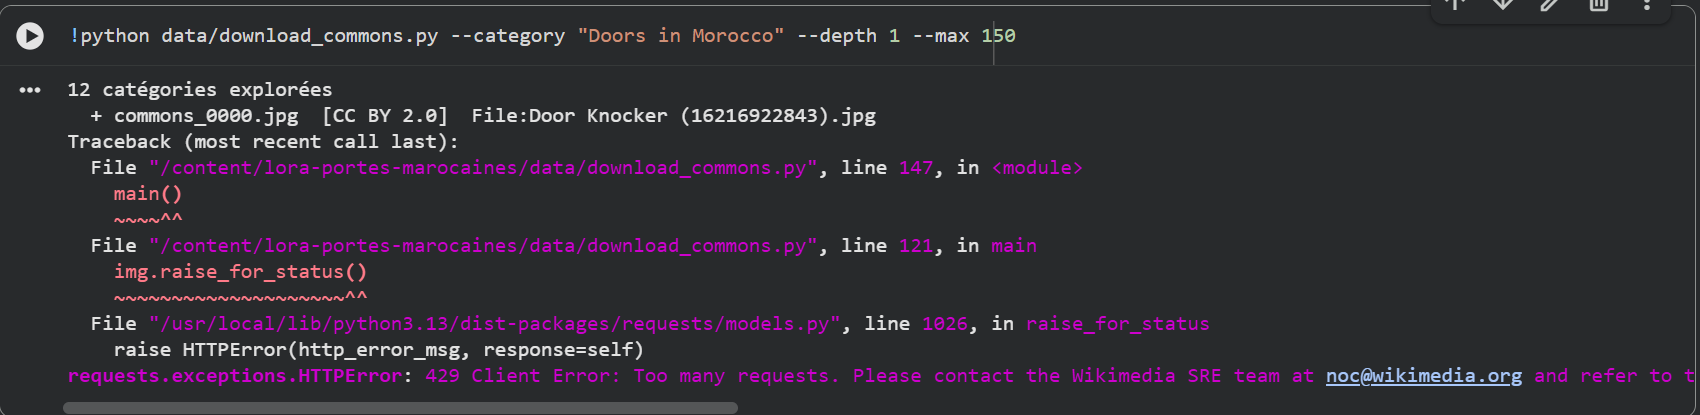
\includegraphics[width=\linewidth]{figures/erreur_429.png}
  \caption{Premier téléchargement depuis Colab : Wikimedia refuse les requêtes trop nombreuses (HTTP~429) dès la deuxième image.}
\end{figure}

\paragraph{Tri manuel.} Une image n'est gardée que si une seule porte est entièrement visible, sans personne, texte ni filigrane. Les 124~images écartées étaient surtout des gros plans de heurtoirs, des coupoles et intérieurs de la mosquée Qarawiyyin, des façades où la porte est petite, et, côté Openverse, des photos militaires renvoyées par le mot « door ». Les titres écartés sont mémorisés pour ne jamais être retéléchargés. Une image a été recadrée pour retirer une personne au bord.

\begin{table}[H]
  \centering
  \caption{Licences des 29 images retenues.}
  \begin{tabular}{lr}
    \toprule
    Licence & Images \\
    \midrule
    CC BY-SA 3.0 & 8 \\
    CC BY-SA 4.0 & 8 \\
    CC BY 2.0 & 7 \\
    CC BY-SA 2.0 & 4 \\
    CC0 / domaine public & 2 \\
    \midrule
    \textbf{Total} & \textbf{29} \\
    \bottomrule
  \end{tabular}
\end{table}

\paragraph{Préparation.} Chaque image est recadrée au centre en $512\times512$ (résolution native de SD~1.5), puis les quasi-doublons sont recherchés par hash perceptuel (dHash) : aucun trouvé. Un découpage fixe (graine~42) réserve 5~images de test jamais vues à l'entraînement ; les 24~autres servent à entraîner.

\paragraph{Légendes.} Chaque image a une légende rédigée à la main sur le modèle \code{a photo of a mrcdoor, <couleur>, <matière>, <décor>}, par exemple « a photo of a mrcdoor, green bronze horseshoe arch door with geometric star patterns, white plaster arch, wall lantern ». Décrire la couleur évite que le modèle associe le mot \trig{} au bleu, très fréquent dans les photos d'Essaouira et de Chefchaouen.

% =====================================================================
\section{Méthode}

Cinq LoRA ont été entraînées puis comparées au modèle de base sur 10~prompts fixes, avec les mêmes graines aléatoires, sur un GPU Tesla~T4 de Kaggle.

\paragraph{Configuration commune.} Stable Diffusion~1.5, LoRA sur l'attention du U-Net (encodeur de texte gelé), taux d'apprentissage $10^{-4}$ constant après 50~étapes de montée, batch effectif~4 (1~image $\times$ 4~accumulations), retournement horizontal aléatoire, graine~42.

\paragraph{Tenir dans la mémoire.} Quatre choix gardent le pic de mémoire GPU vers 2~Go, six fois sous la limite de 12~Go du sujet :
\begin{itemize}
  \item poids gelés en fp16, seuls $A$ et $B$ en fp32 avec précision mixte ;
  \item gradient checkpointing (on recalcule les activations au lieu de les stocker) ;
  \item latents et embeddings de texte calculés une seule fois, puis VAE et CLIP retirés du GPU ;
  \item accumulation de gradients au lieu d'un vrai batch de~4.
\end{itemize}

\paragraph{Plan d'expériences.}
\begin{enumerate}
  \item Rangs 4, 8, 16 et 32, à 1\,000~étapes chacun, évalués aux intensités 0,5, 0,8 et 1,0.
  \item Rang~8 entraîné 2\,000~étapes, avec une sauvegarde toutes les 250~étapes, pour suivre l'évolution.
\end{enumerate}

\paragraph{Prompts d'évaluation.} 4~prompts du domaine (« a mrcdoor with blue zellige tiles around it »\ldots), 4 de généralisation qui placent le concept dans un contexte absent des données (neige, bâtiment de verre, porte rouge la nuit, aquarelle) et 2~prompts « de fuite » sans le mot déclencheur (un chat, une cuisine). Chaque prompt est généré avec 4~graines (2 pour la série d'étapes), 30~étapes de débruitage, guidance~7,5.

\paragraph{Métriques.} Toutes reposent sur les embeddings de CLIP ViT-B/32 (similarité cosinus).

\begin{table}[H]
  \centering
  \caption{Métriques d'évaluation.}
  \small
  \begin{tabularx}{\linewidth}{l Y l}
    \toprule
    Métrique & Ce qu'elle mesure & Lecture \\
    \midrule
    CLIPScore & accord image $\leftrightarrow$ prompt (« mrcdoor » remplacé par « moroccan door », que CLIP comprend) & plus haut = mieux \\
    Proximité au domaine & image générée $\leftrightarrow$ les 5 vraies portes de test & plus haut = plus fidèle \\
    Taux de copie & part des images à plus de 0,95 de similarité avec une image d'entraînement & 0~\% = aucune copie \\
    Diversité & $1 -$ similarité moyenne entre graines d'un même prompt & plus bas = trop semblables \\
    Fuite de style & image avec LoRA $\leftrightarrow$ image du modèle de base, prompts sans déclencheur & 1 = aucune contamination \\
    \bottomrule
  \end{tabularx}
\end{table}

\paragraph{Pourquoi pas la FID.} La FID compare deux distributions et demande des milliers d'images réelles ; avec 5~images de test elle n'aurait aucune valeur statistique.

\paragraph{Pourquoi pas la perte.} Les courbes de perte des cinq entraînements sont presque identiques (écart final $< 0{,}003$) et ne baissent pas nettement : en diffusion, la perte dépend surtout du niveau de bruit tiré au hasard à chaque étape. Elle ne dit rien de la qualité, d'où l'évaluation sur les images générées.

% =====================================================================
\section{Résultats}

Toutes les LoRA améliorent le modèle de base, et le rang~16 à 1\,000~étapes offre le meilleur compromis : même qualité que le rang~32 pour un fichier deux fois plus léger. Chaque valeur est une moyenne sur 16~images (4~prompts $\times$ 4~graines) : les écarts de moins d'environ 0,5~point de CLIPScore sont à lire comme des tendances, pas comme des différences certaines.

\subsection{Coût}

L'entraînement complet a pris 155~minutes de GPU~T4, avec un pic de mémoire de 2,13~Go. Le rang ne change presque rien au temps ni à la mémoire : il ne joue que sur la taille du fichier.

\begin{table}[H]
  \centering
  \caption{Coût de chaque entraînement.}
  \small
  \begin{tabular}{lrrrrr}
    \toprule
    LoRA & Paramètres & \shortstack[r]{Part du\\U-Net} & \shortstack[r]{Temps\\(min)} & \shortstack[r]{Mémoire\\max (Go)} & \shortstack[r]{Fichier\\(Mo)} \\
    \midrule
    Rang 4 & 0,80 M & 0,09 \% & 25,7 & 2,04 & 3,2 \\
    Rang 8 & 1,59 M & 0,19 \% & 25,7 & 2,06 & 6,4 \\
    \rowcolor{bleu!10} Rang 16 & 3,19 M & 0,37 \% & 25,8 & 2,08 & 12,8 \\
    Rang 32 & 6,38 M & 0,74 \% & 25,9 & 2,13 & 25,6 \\
    Rang 8, 2\,000 étapes & 1,59 M & 0,19 \% & 52,1 & 2,06 & 6,4 \\
    \bottomrule
  \end{tabular}
\end{table}

Le modèle complet pèse 3,4~Go : la LoRA de rang~16 en représente 0,4~\%. La génération coûte 6,0~s par image avec LoRA contre 5,6~s sans.

\begin{figure}[H]
  \centering
  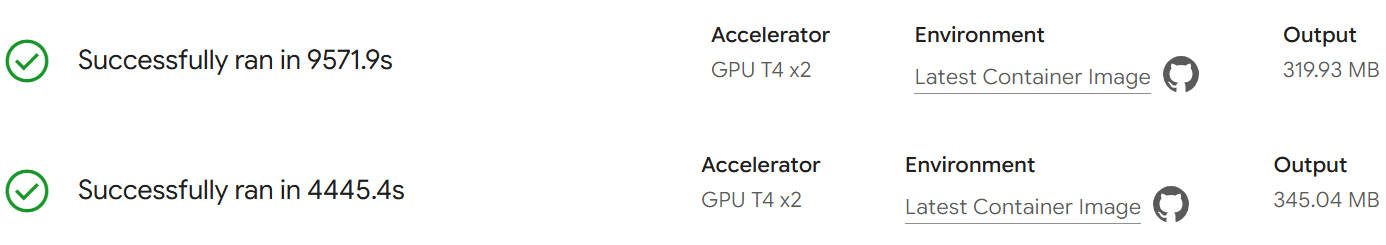
\includegraphics[width=0.85\linewidth]{figures/runs_kaggle.png}
  \caption{Exécutions Kaggle : entraînement des cinq LoRA (9\,572~s, environ 2~h~40) puis évaluation (4\,445~s, environ 1~h~14), sur GPU~T4.}
\end{figure}

\subsection{Comparaison des rangs (Q1)}

Intensité 1,0, 1\,000~étapes. « Domaine » et « généralisation » désignent les deux groupes de prompts.

\begin{table}[H]
  \centering
  \caption{Comparaison des rangs.}
  \small
  \begin{tabular}{lrrrr}
    \toprule
    Modèle & \shortstack[r]{CLIPScore\\domaine} & \shortstack[r]{Proximité\\domaine} & \shortstack[r]{CLIPScore\\généralisation} & \shortstack[r]{Fuite\\(1 = aucune)} \\
    \midrule
    Base, sans LoRA & 31,5 & 0,731 & 29,4 & 1,00 \\
    Rang 4 & 33,3 & 0,752 & 30,6 & 0,91 \\
    Rang 8 & 35,0 & 0,764 & 30,8 & 0,92 \\
    \rowcolor{bleu!10} \textbf{Rang 16} & \textbf{35,2} & \textbf{0,788} & \textbf{31,5} & 0,92 \\
    Rang 32 & 35,3 & 0,783 & 31,5 & 0,93 \\
    \bottomrule
  \end{tabular}
\end{table}

Le rang~4 est nettement en dessous des autres ; au-delà du rang~16, la qualité plafonne alors que le fichier double. Aucune configuration ne recopie ses images d'entraînement : le taux de copie vaut 0~\% partout.

\subsection{Intensité de la LoRA}

Monter l'intensité renforce le style mais augmente la fuite vers les prompts qui ne parlent pas de portes. Exemple au rang~16 :

\begin{table}[H]
  \centering
  \caption{Effet de l'intensité, rang 16.}
  \small
  \begin{tabular}{rrrr}
    \toprule
    Intensité & CLIPScore domaine & Proximité domaine & Fuite (1 = aucune) \\
    \midrule
    0,5 & 33,4 & 0,772 & 0,96 \\
    \rowcolor{bleu!10} 0,8 & 34,7 & 0,779 & 0,94 \\
    1,0 & 35,2 & 0,788 & 0,92 \\
    \bottomrule
  \end{tabular}
\end{table}

La même tendance se retrouve aux quatre rangs. Une intensité de 0,8 garde l'essentiel du gain tout en limitant la contamination.

\subsection{Nombre d'étapes (Q2)}

La qualité progresse jusqu'à 1\,250~étapes, puis stagne : continuer jusqu'à 2\,000~étapes double le temps d'entraînement sans gain. Nous n'observons pas de surapprentissage net : aucune copie des images d'entraînement, et une diversité sous celle du modèle de base à 7~points sur~8, mais trop variable (2~graines par prompt) pour montrer une tendance.

\begin{figure}[H]
  \centering
  \begin{tikzpicture}
    \begin{axis}[
      name=haut,
      width=0.92\linewidth, height=5.2cm,
      title={\small CLIPScore (respect du texte), prompts du domaine},
      xmin=150, xmax=2100, ymin=31, ymax=36.8,
      xtick={250,500,750,1000,1250,1500,1750,2000},
      xticklabels={},
      ylabel={CLIPScore},
      grid=major, grid style={gray!20},
      every axis plot/.append style={thick},
      tick label style={font=\small},
      /pgf/number format/use comma,
    ]
      \addplot[color=bleu, mark=*] coordinates {
        (250,33.56) (500,34.34) (750,34.49) (1000,35.53)
        (1250,36.16) (1500,35.64) (1750,35.10) (2000,35.44)};
      \addplot[color=gris, dashed, domain=150:2100] {31.69};
      \node[font=\scriptsize, color=gris, anchor=south east] at (axis cs:2080,31.69) {base 31,7};
      \node[font=\scriptsize, color=terre, anchor=south] at (axis cs:1250,36.16) {36,2 à 1\,250 étapes};
    \end{axis}
    \begin{axis}[
      at={(haut.south)}, anchor=north, yshift=-1.3cm,
      width=0.92\linewidth, height=4.6cm,
      title={\small Diversité entre graines (plus bas = images plus semblables)},
      xmin=150, xmax=2100, ymin=0.08, ymax=0.16,
      xtick={250,500,750,1000,1250,1500,1750,2000},
      xlabel={Étapes d'entraînement},
      ylabel={Diversité},
      grid=major, grid style={gray!20},
      every axis plot/.append style={thick},
      tick label style={font=\small},
      yticklabel style={/pgf/number format/fixed,/pgf/number format/precision=2,/pgf/number format/use comma},
      xticklabel style={/pgf/number format/1000 sep={\,}},
    ]
      \addplot[color=terre, mark=*] coordinates {
        (250,0.1085) (500,0.1188) (750,0.1469) (1000,0.1044)
        (1250,0.1148) (1500,0.0927) (1750,0.1239) (2000,0.1029)};
      \addplot[color=gris, dashed, domain=150:2100] {0.132};
      \node[font=\scriptsize, color=gris, anchor=south east] at (axis cs:2080,0.132) {base 0,132};
    \end{axis}
  \end{tikzpicture}
  \caption{Rang 8, 8 sauvegardes de 250 à 2\,000 étapes (\code{results/eval\_etapes/metrics.csv}). La qualité plafonne vers 1\,250 étapes.}
\end{figure}

% =====================================================================
\section{Analyse qualitative (Q3)}

La LoRA reproduit bien le style des portes marocaines dans leur décor naturel, mais le concept s'efface dès que le prompt impose un contexte trop éloigné des photos d'entraînement.

Avec la même graine, les quatre rangs donnent la même composition (cadrage, position de la porte) : la LoRA modifie les détails et le style, pas la mise en page. Les observations ci-dessous viennent des grilles de \code{results/eval/} et \code{results/eval\_etapes/} (une ligne par prompt, une colonne par graine).

\begin{figure}[p]
  \centering
  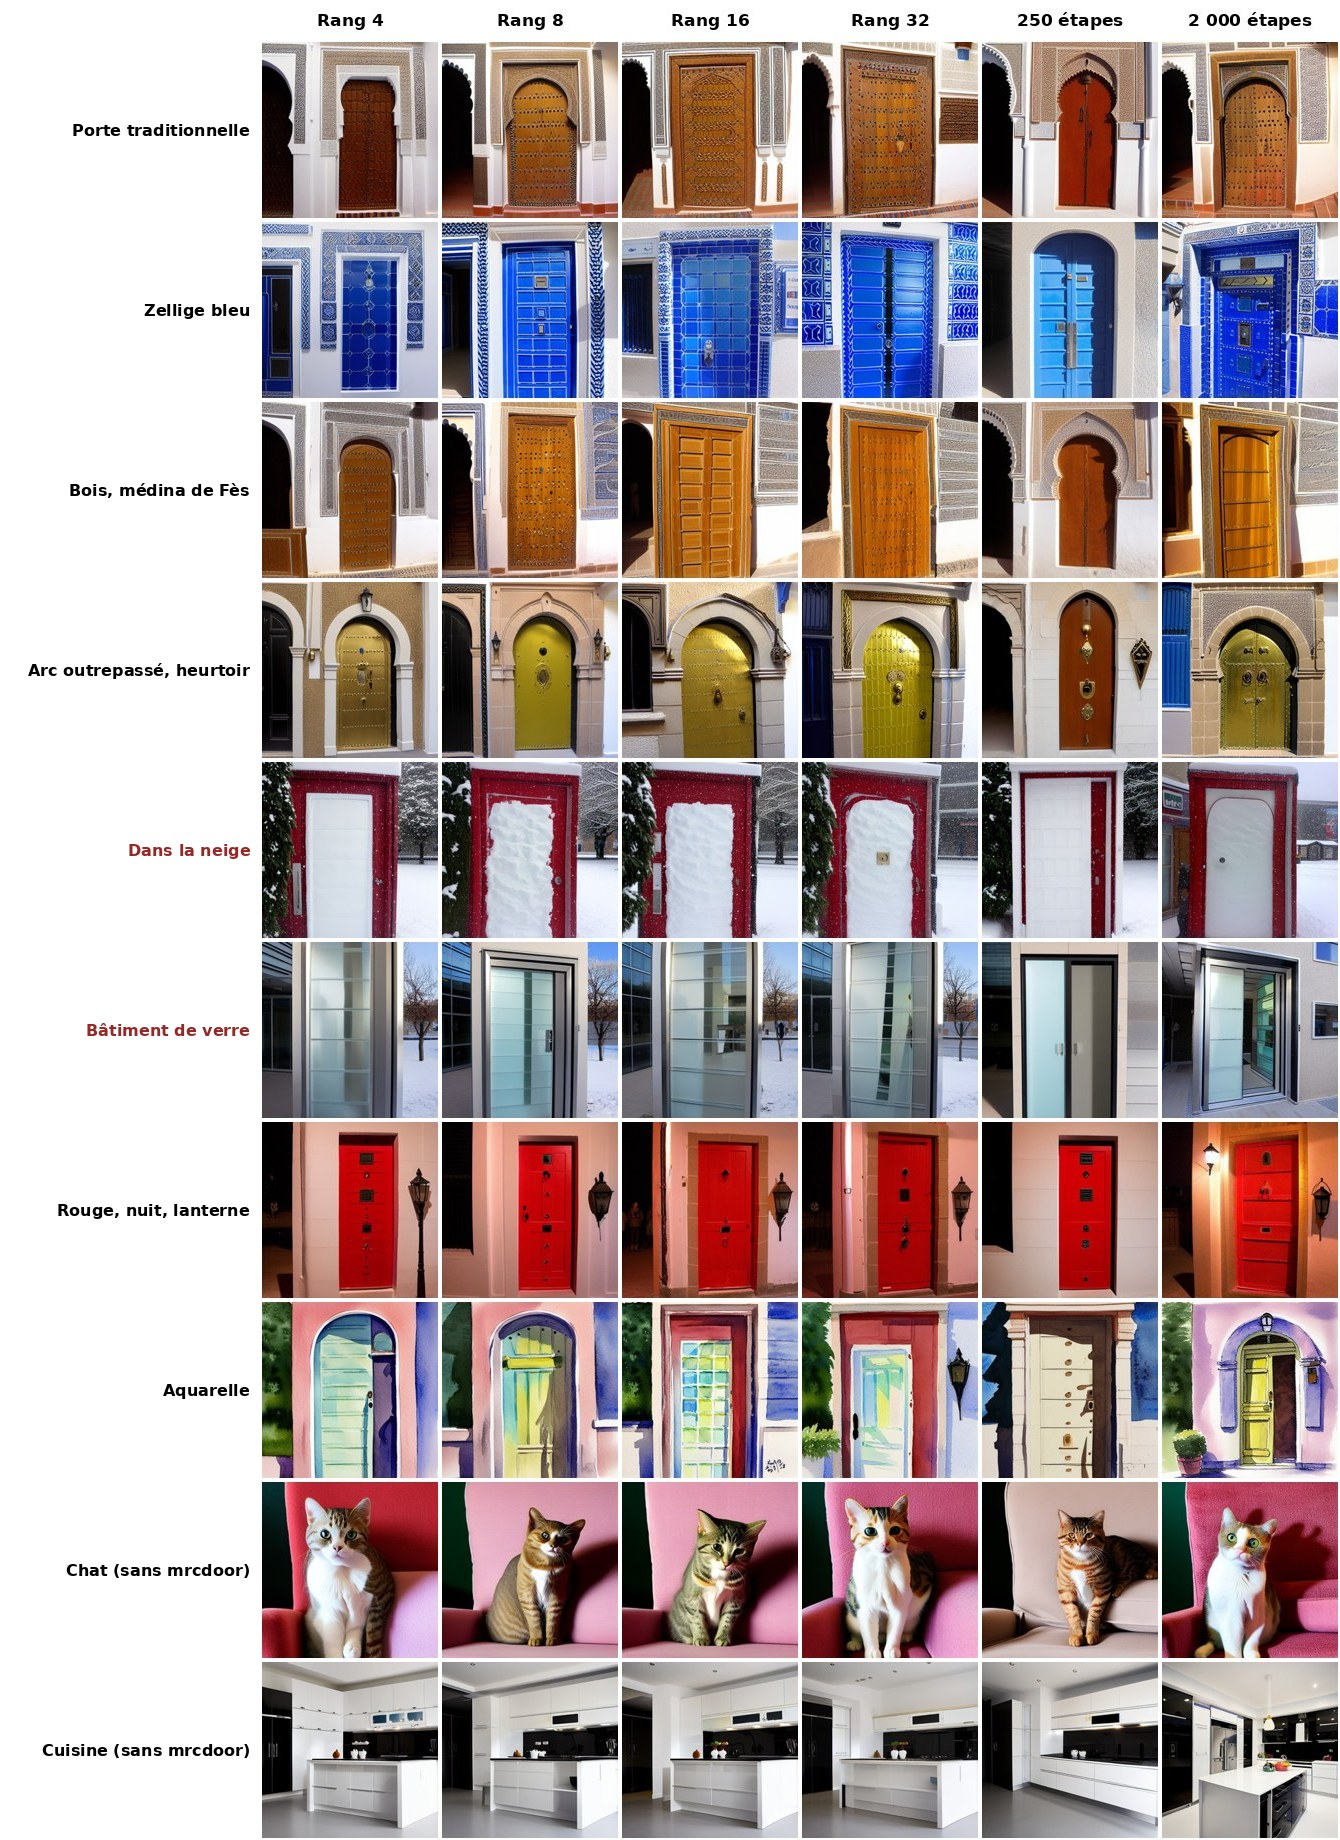
\includegraphics[height=0.88\textheight]{figures/planche_qualitative.jpg}
  \caption{Première graine de chaque prompt, intensité 1,0 : quatre rangs à 1\,000 étapes, puis le rang 8 à 250 et 2\,000 étapes. En rouge, les deux contextes où le concept disparaît.}
\end{figure}

\subsection*{Réussites}
\begin{enumerate}
  \item \textbf{Le style du domaine.} Sur les 4~prompts du domaine, toutes les LoRA produisent des cadres sculptés, des arcs outrepassés, du cloutage et du zellige. Le style apparaît dès 250~étapes ; à 2\,000~étapes, les détails (clous, carreaux) sont plus nombreux.
  \item \textbf{Les attributs restent contrôlables.} « A red mrcdoor at night, lit by a lantern » donne bien des portes rouges avec une lanterne, alors qu'aucune porte rouge n'était dans les données. Décrire la couleur dans les légendes a donc fonctionné : le mot \trig{} n'a pas absorbé le bleu.
  \item \textbf{Un style pictural.} « A watercolor painting of a mrcdoor » produit des aquarelles avec arc et encadrement marocains, le plus nettement à 2\,000~étapes.
\end{enumerate}

\subsection*{Échecs}
\begin{enumerate}
  \item \textbf{Le bâtiment moderne.} « A mrcdoor on a modern glass building » donne des portes vitrées sans aucun trait marocain, à tous les rangs et toutes les étapes : le contexte écrase le concept.
  \item \textbf{La neige.} « A mrcdoor in the snow » donne bien la neige, mais la porte devient générique (cadre rouge, battant blanc) et perd sculptures et arc.
  \item \textbf{Le zellige envahissant.} Avec « blue zellige tiles around it », les carreaux débordent parfois sur la porte elle-même, qui finit entièrement carrelée : le modèle mélange l'objet et son décor.
  \item \textbf{Une fuite légère.} Les chats et les cuisines restent des chats et des cuisines, avec la même composition, mais leurs couleurs et textures changent un peu (similarité 0,91 à 0,96 avec le modèle de base).
\end{enumerate}

\subsection*{Pourquoi ces échecs}
Les 24~photos montrent toutes une porte de face, de jour, dans une médina, et toutes les légendes commencent par « a photo of ». Le modèle a donc appris « porte marocaine photographiée dans sa rue » plutôt qu'un objet détachable de son décor. L'encodeur de texte étant gelé, le mot \trig{} pèse peu face à des mots très forts comme « modern glass building ». Trois pistes y répondraient : des images de régularisation (\emph{prior preservation}, qui limite aussi la fuite), des légendes plus variées, et une LoRA sur l'encodeur de texte.

\subsection*{Démo interactive}
Une interface Gradio (\code{demo/app.py}, lancée sur Kaggle par \code{scripts/demo\_kaggle.py}) génère deux images avec le même prompt et la même seed : l'une avec le modèle de base, l'autre avec la LoRA. On choisit le rang, l'intensité et le nombre d'étapes. Avec la configuration recommandée (rang~16, intensité~0,8), une image prend environ 4,5~s sur~T4.

\begin{figure}[H]
  \centering
  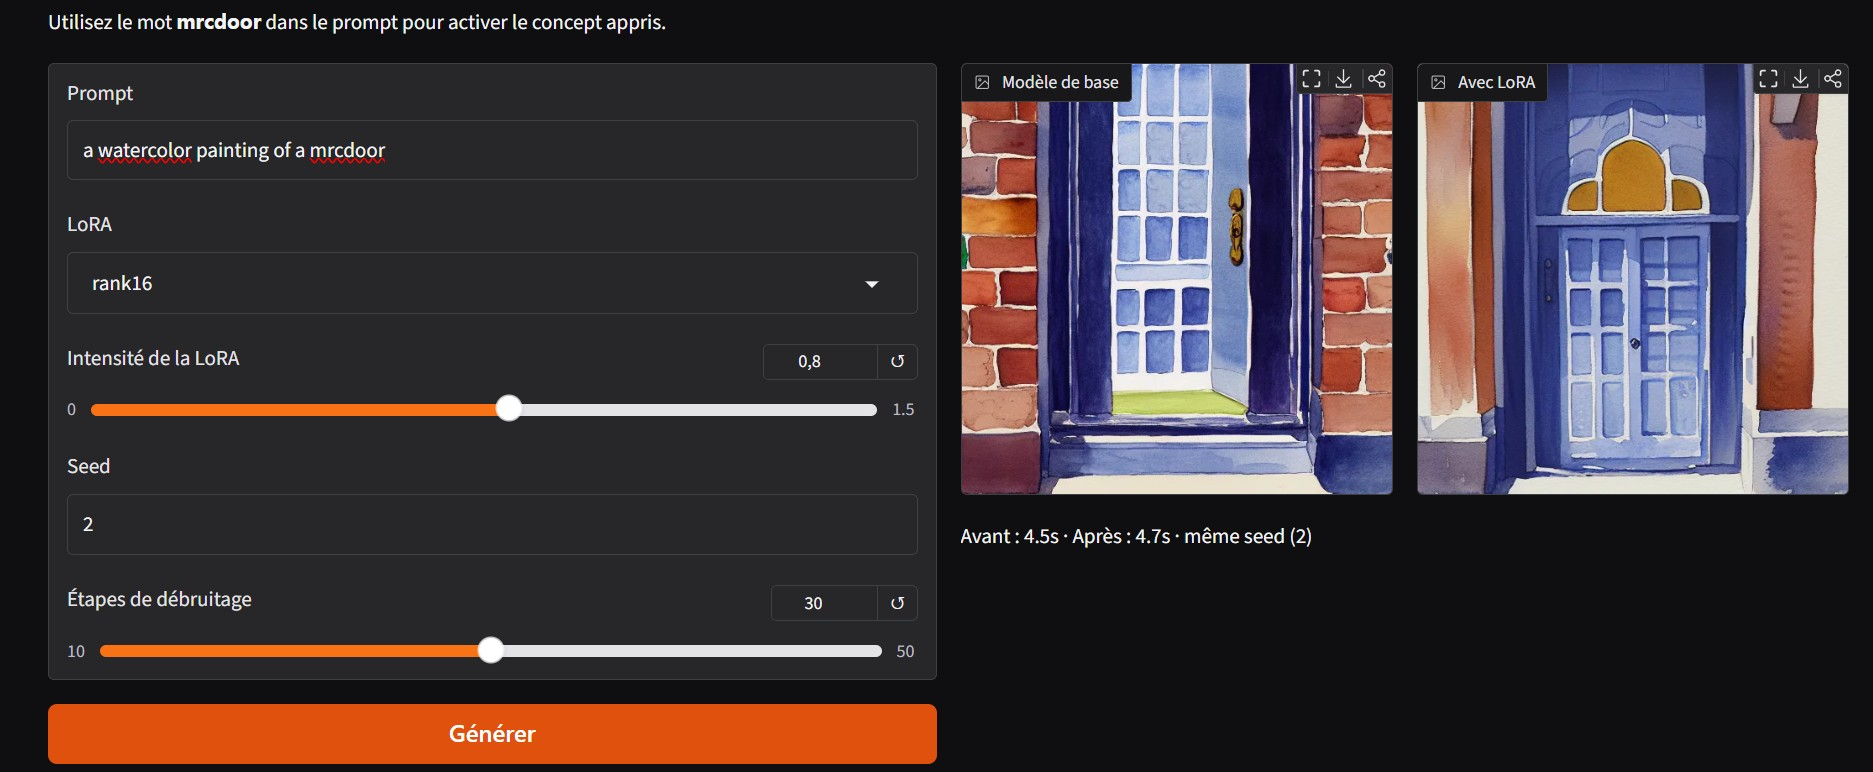
\includegraphics[width=\linewidth]{figures/demo_seed2.jpg}
  \caption{Démo, seed 2. Le modèle de base ne connaît pas « mrcdoor » et dessine une porte européenne entre des murs de briques. Avec la LoRA, on obtient un arc polylobé, du bleu profond et des murs ocre rosé. Toutes les seeds ne donnent pas un résultat aussi net : sur les seeds 0 et 1, l'image change mais sans arc reconnaissable, ce qui rejoint les échecs décrits plus haut.}
\end{figure}

% =====================================================================
\section{Éthique et limites}

\paragraph{Droits.} Les 29~images sont sous CC0, CC~BY ou CC~BY-SA, avec auteur et lien dans \code{data/sources.csv} ; les crédits complets figurent dans \code{docs/licences.md}. 20~images sont sous CC~BY-SA, qui demande de partager les œuvres dérivées sous la même licence. Savoir si un modèle entraîné en est une reste débattu ; par prudence, nous publions la LoRA sous CC~BY-SA~4.0. Aucun artiste vivant n'est ciblé et aucun nom d'artiste n'apparaît dans les prompts.

\paragraph{Patrimoine.} Le zellige et la menuiserie sculptée sont un savoir-faire artisanal vivant. Des images générées en masse peuvent concurrencer artisans et photographes, et le modèle mélange des motifs de villes et d'époques différentes : ses images ne doivent pas servir de référence historique. La démo les signale comme générées.

\paragraph{Personnes.} Les photos montrant des personnes ont été écartées au tri, et une image recadrée, pour respecter le droit à l'image et éviter que la LoRA n'apprenne des visages.

\paragraph{Limites de l'étude.}
\begin{itemize}
  \item 29~images, dont seulement 5 pour le test : les métriques de proximité reposent sur très peu de références.
  \item Le jeu est biaisé vers Essaouira et les portes de la mosquée Qarawiyyin de Fès, souvent photographiées par les mêmes auteurs ; Rabat, Tétouan ou Marrakech sont peu représentées.
  \item Chaque chiffre repose sur 16~images (8 pour la série d'étapes) : les petits écarts entre rangs sont fragiles.
  \item CLIP juge le respect du texte à travers « moroccan door » : il ne voit pas les détails fins que l'œil d'un artisan repèrerait.
  \item Le seuil de copie (0,95) est un choix ; abaissé, il pourrait révéler des quasi-copies.
\end{itemize}

\paragraph{Coût énergétique.} Le projet a consommé environ 3~h~50 de GPU~T4 : 155~minutes d'entraînement et 74~minutes d'évaluation.

% =====================================================================
\section{Conclusion}

Avec 24~photos et 26~minutes de GPU gratuit, une LoRA de rang~16 apprend le style des portes marocaines sans recopier ses données, mais ne le transpose pas encore dans des contextes très éloignés.

\begin{itemize}
  \item \textbf{Q1 --- Rang.} Le rang~16 est le meilleur compromis : CLIPScore 35,2 et proximité 0,788, autant que le rang~32 pour un fichier de 12,8~Mo au lieu de 25,6. Le rang~4 est trop limité.
  \item \textbf{Q2 --- Étapes.} La qualité plafonne vers 1\,250~étapes ; au-delà, on ne gagne plus rien. Sur 2\,000~étapes, nous n'observons pas de surapprentissage net : aucune copie, et une diversité trop variable pour conclure.
  \item \textbf{Q3 --- Généralisation.} Partielle : couleur et style pictural se combinent bien avec le concept, mais un bâtiment moderne ou la neige l'effacent. Une intensité de 0,8 limite la fuite vers les prompts sans rapport.
\end{itemize}

\begin{center}
\fcolorbox{bleu}{bleu!6}{\parbox{0.9\linewidth}{\centering\textbf{Configuration recommandée :} rang 16, 1\,000 à 1\,250 étapes, intensité 0,8 à la génération.}}
\end{center}

\paragraph{Pistes.} Des images de régularisation contre la fuite, une LoRA sur l'encodeur de texte pour renforcer le mot déclencheur, des légendes et des photos plus variées (portes de Rabat prises par l'équipe, vues de nuit), et un passage à SDXL si la mémoire le permet.

\end{document}
